\documentclass[a4paper,12pt]{article}
\usepackage[margin=18mm]{geometry}
\usepackage{tikz}
\usepackage{amsmath}
\usepackage{xcolor}
\newcommand{\pFourCell}[2]{\makebox[#1em][c]{\ensuremath{#2}}}
\newcommand{\pFourCenterBox}[1]{\begingroup\setbox0=\hbox{$\displaystyle #1$}\dimen0=\ht0\advance\dimen0 by -\dp0\divide\dimen0 by 2\lower\dimen0\box0\endgroup}
\newdimen\pFourFractionRuleThickness
\pFourFractionRuleThickness=0.4pt
\newcommand{\pFourTopAlign}[3]{\raisebox{-#1}[0pt][\dimexpr #1 + #2\relax]{\ensuremath{\displaystyle #3}}}
\newcommand{\pFourBottomAlign}[3]{\raisebox{#2}[\dimexpr #1 + #2\relax][0pt]{\ensuremath{\displaystyle #3}}}
\newcommand{\pFourFractionInner}[2]{\hbox to #1{\hss$\displaystyle #2$\hss}}
\newcommand{\pFourFractionC}[4]{\begingroup\color{#1}\genfrac{}{}{\pFourFractionRuleThickness}{0}{\raisebox{0.14em}{\pFourFractionInner{#2}{{\color{black}#3}}}}{\raisebox{-0.18em}{\pFourFractionInner{#2}{{\color{black}#4}}}}\endgroup}
\newcommand{\pFourFraction}[3]{\genfrac{}{}{\pFourFractionRuleThickness}{0}{\raisebox{0.14em}{\pFourFractionInner{#1}{#2}}}{\raisebox{-0.18em}{\pFourFractionInner{#1}{#3}}}}
\newcommand{\pFourRootC}[2]{\begingroup\setbox0=\hbox{$\displaystyle #2$}\setbox2=\hbox{$\displaystyle \sqrt{\phantom{\copy0}}$}\dimen0=\wd2\advance\dimen0 by -\wd0\hbox{\rlap{\textcolor{#1}{\copy2}}\kern\dimen0\box0}\endgroup}
\newcommand{\pFourRoot}[1]{\pFourRootC{black}{#1}}
\newcommand{\pFourRootDegreeC}[3]{\begingroup\setbox0=\hbox{$\displaystyle #3$}\setbox2=\hbox{$\displaystyle \sqrt[#2]{\phantom{\copy0}}$}\dimen0=\wd2\advance\dimen0 by -\wd0\hbox{\rlap{\textcolor{#1}{\copy2}}\kern\dimen0\box0}\endgroup}
\newcommand{\pFourRootDegree}[2]{\pFourRootDegreeC{black}{#1}{#2}}
\pagestyle{empty}
\begin{document}

\section*{Spaltentreue LaTeX-Ausgabe}
\noindent Gleichung: \texttt{y}\texttt{=}\texttt{a}\texttt{*}\texttt{B}\texttt{\textasciicircum{}}\texttt{x} \hfill Zielvariable: \texttt{x} \hfill Profil: \texttt{standard}

\vspace{8mm}
\begin{center}
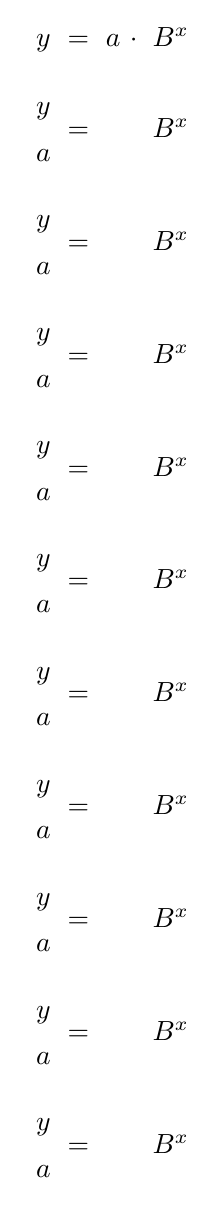
\begin{tikzpicture}[x=1em,y=-1em]
\node[anchor=base, inner sep=0pt] at (0.45,1.87) {$\pFourCell{0.9}{y}$};
\node[anchor=base, inner sep=0pt] at (1.71,1.87) {$\pFourCell{1.62}{=}$};
\node[anchor=base, inner sep=0pt] at (2.97,1.87) {$\pFourCell{0.9}{a}$};
\node[anchor=base, inner sep=0pt] at (3.71,1.87) {$\pFourCell{0.58}{\cdot}$};
\node[anchor=base, inner sep=0pt] at (5.05,1.87) {$B^{{\scriptstyle x}}$};
\node[anchor=base, inner sep=0pt] at (0.45,5.15) {$\pFourFraction{0.9em}{\pFourCell{0.9}{y}}{\pFourCell{0.9}{a}}$};
\node[anchor=base, inner sep=0pt] at (1.71,5.15) {$\pFourCell{1.62}{=}$};
\node[anchor=base, inner sep=0pt] at (5.05,5.15) {$B^{{\scriptstyle x}}$};
\node[anchor=base, inner sep=0pt] at (0.45,9.23) {$\pFourFraction{0.9em}{\pFourCell{0.9}{y}}{\pFourCell{0.9}{a}}$};
\node[anchor=base, inner sep=0pt] at (1.71,9.23) {$\pFourCell{1.62}{=}$};
\node[anchor=base, inner sep=0pt] at (5.05,9.23) {$B^{{\scriptstyle x}}$};
\node[anchor=base, inner sep=0pt] at (0.45,13.31) {$\pFourFraction{0.9em}{\pFourCell{0.9}{y}}{\pFourCell{0.9}{a}}$};
\node[anchor=base, inner sep=0pt] at (1.71,13.31) {$\pFourCell{1.62}{=}$};
\node[anchor=base, inner sep=0pt] at (5.05,13.31) {$B^{{\scriptstyle x}}$};
\node[anchor=base, inner sep=0pt] at (0.45,17.39) {$\pFourFraction{0.9em}{\pFourCell{0.9}{y}}{\pFourCell{0.9}{a}}$};
\node[anchor=base, inner sep=0pt] at (1.71,17.39) {$\pFourCell{1.62}{=}$};
\node[anchor=base, inner sep=0pt] at (5.05,17.39) {$B^{{\scriptstyle x}}$};
\node[anchor=base, inner sep=0pt] at (0.45,21.47) {$\pFourFraction{0.9em}{\pFourCell{0.9}{y}}{\pFourCell{0.9}{a}}$};
\node[anchor=base, inner sep=0pt] at (1.71,21.47) {$\pFourCell{1.62}{=}$};
\node[anchor=base, inner sep=0pt] at (5.05,21.47) {$B^{{\scriptstyle x}}$};
\node[anchor=base, inner sep=0pt] at (0.45,25.55) {$\pFourFraction{0.9em}{\pFourCell{0.9}{y}}{\pFourCell{0.9}{a}}$};
\node[anchor=base, inner sep=0pt] at (1.71,25.55) {$\pFourCell{1.62}{=}$};
\node[anchor=base, inner sep=0pt] at (5.05,25.55) {$B^{{\scriptstyle x}}$};
\node[anchor=base, inner sep=0pt] at (0.45,29.63) {$\pFourFraction{0.9em}{\pFourCell{0.9}{y}}{\pFourCell{0.9}{a}}$};
\node[anchor=base, inner sep=0pt] at (1.71,29.63) {$\pFourCell{1.62}{=}$};
\node[anchor=base, inner sep=0pt] at (5.05,29.63) {$B^{{\scriptstyle x}}$};
\node[anchor=base, inner sep=0pt] at (0.45,33.71) {$\pFourFraction{0.9em}{\pFourCell{0.9}{y}}{\pFourCell{0.9}{a}}$};
\node[anchor=base, inner sep=0pt] at (1.71,33.71) {$\pFourCell{1.62}{=}$};
\node[anchor=base, inner sep=0pt] at (5.05,33.71) {$B^{{\scriptstyle x}}$};
\node[anchor=base, inner sep=0pt] at (0.45,37.79) {$\pFourFraction{0.9em}{\pFourCell{0.9}{y}}{\pFourCell{0.9}{a}}$};
\node[anchor=base, inner sep=0pt] at (1.71,37.79) {$\pFourCell{1.62}{=}$};
\node[anchor=base, inner sep=0pt] at (5.05,37.79) {$B^{{\scriptstyle x}}$};
\node[anchor=base, inner sep=0pt] at (0.45,41.87) {$\pFourFraction{0.9em}{\pFourCell{0.9}{y}}{\pFourCell{0.9}{a}}$};
\node[anchor=base, inner sep=0pt] at (1.71,41.87) {$\pFourCell{1.62}{=}$};
\node[anchor=base, inner sep=0pt] at (5.05,41.87) {$B^{{\scriptstyle x}}$};
\end{tikzpicture}
\end{center}


\newpage
\section*{Spaltentreue LaTeX-Ausgabe mit Spaltengrenzen}
\vspace{6mm}
\begin{center}
\begin{tikzpicture}[x=1em,y=-1em]
\node[font={\scriptsize}, text=gray!65, anchor=west] at (0,-0.75) {Spaltengrenzen: blau; Spaltenmitten: grau gepunktet; lokale Bruch-/Span-Achsen: rot};
\draw[blue!22, line width=0.28pt] (0,0.35) -- (0,44.15);
\draw[blue!22, line width=0.28pt] (0.9,0.35) -- (0.9,44.15);
\draw[blue!22, line width=0.28pt] (2.52,0.35) -- (2.52,44.15);
\draw[blue!22, line width=0.28pt] (3.42,0.35) -- (3.42,44.15);
\draw[blue!22, line width=0.28pt] (4,0.35) -- (4,44.15);
\draw[blue!22, line width=0.28pt] (6.1,0.35) -- (6.1,44.15);
\draw[gray!35, dotted] (0.45,0.35) -- (0.45,44.15);
\node[font={\ttfamily\scriptsize}, text=gray!70, anchor=base] at (0.45,0) {0};
\draw[gray!35, dotted] (1.71,0.35) -- (1.71,44.15);
\node[font={\ttfamily\scriptsize}, text=gray!70, anchor=base] at (1.71,0) {1};
\draw[gray!35, dotted] (2.97,0.35) -- (2.97,44.15);
\node[font={\ttfamily\scriptsize}, text=gray!70, anchor=base] at (2.97,0) {2};
\draw[gray!35, dotted] (3.71,0.35) -- (3.71,44.15);
\node[font={\ttfamily\scriptsize}, text=gray!70, anchor=base] at (3.71,0) {3};
\draw[gray!35, dotted] (5.05,0.35) -- (5.05,44.15);
\node[font={\ttfamily\scriptsize}, text=gray!70, anchor=base] at (5.05,0) {4};
\node[anchor=base, inner sep=0pt] at (0.45,1.87) {$\pFourCell{0.9}{y}$};
\node[anchor=base, inner sep=0pt] at (1.71,1.87) {$\pFourCell{1.62}{=}$};
\node[anchor=base, inner sep=0pt] at (2.97,1.87) {$\pFourCell{0.9}{a}$};
\node[anchor=base, inner sep=0pt] at (3.71,1.87) {$\pFourCell{0.58}{\cdot}$};
\node[anchor=base, inner sep=0pt] at (5.05,1.87) {$B^{{\scriptstyle x}}$};
\draw[red!30, opacity=0.32, line width=0.35pt] (0.45,3.4) -- (0.45,6.53);
\node[anchor=base, inner sep=0pt] at (0.45,5.15) {$\pFourFraction{0.9em}{\pFourCell{0.9}{y}}{\pFourCell{0.9}{a}}$};
\node[anchor=base, inner sep=0pt] at (1.71,5.15) {$\pFourCell{1.62}{=}$};
\node[anchor=base, inner sep=0pt] at (5.05,5.15) {$B^{{\scriptstyle x}}$};
\draw[red!30, opacity=0.32, line width=0.35pt] (0.45,7.48) -- (0.45,10.61);
\node[anchor=base, inner sep=0pt] at (0.45,9.23) {$\pFourFraction{0.9em}{\pFourCell{0.9}{y}}{\pFourCell{0.9}{a}}$};
\node[anchor=base, inner sep=0pt] at (1.71,9.23) {$\pFourCell{1.62}{=}$};
\node[anchor=base, inner sep=0pt] at (5.05,9.23) {$B^{{\scriptstyle x}}$};
\draw[red!30, opacity=0.32, line width=0.35pt] (0.45,11.56) -- (0.45,14.69);
\node[anchor=base, inner sep=0pt] at (0.45,13.31) {$\pFourFraction{0.9em}{\pFourCell{0.9}{y}}{\pFourCell{0.9}{a}}$};
\node[anchor=base, inner sep=0pt] at (1.71,13.31) {$\pFourCell{1.62}{=}$};
\node[anchor=base, inner sep=0pt] at (5.05,13.31) {$B^{{\scriptstyle x}}$};
\draw[red!30, opacity=0.32, line width=0.35pt] (0.45,15.64) -- (0.45,18.77);
\node[anchor=base, inner sep=0pt] at (0.45,17.39) {$\pFourFraction{0.9em}{\pFourCell{0.9}{y}}{\pFourCell{0.9}{a}}$};
\node[anchor=base, inner sep=0pt] at (1.71,17.39) {$\pFourCell{1.62}{=}$};
\node[anchor=base, inner sep=0pt] at (5.05,17.39) {$B^{{\scriptstyle x}}$};
\draw[red!30, opacity=0.32, line width=0.35pt] (0.45,19.72) -- (0.45,22.85);
\node[anchor=base, inner sep=0pt] at (0.45,21.47) {$\pFourFraction{0.9em}{\pFourCell{0.9}{y}}{\pFourCell{0.9}{a}}$};
\node[anchor=base, inner sep=0pt] at (1.71,21.47) {$\pFourCell{1.62}{=}$};
\node[anchor=base, inner sep=0pt] at (5.05,21.47) {$B^{{\scriptstyle x}}$};
\draw[red!30, opacity=0.32, line width=0.35pt] (0.45,23.8) -- (0.45,26.93);
\node[anchor=base, inner sep=0pt] at (0.45,25.55) {$\pFourFraction{0.9em}{\pFourCell{0.9}{y}}{\pFourCell{0.9}{a}}$};
\node[anchor=base, inner sep=0pt] at (1.71,25.55) {$\pFourCell{1.62}{=}$};
\node[anchor=base, inner sep=0pt] at (5.05,25.55) {$B^{{\scriptstyle x}}$};
\draw[red!30, opacity=0.32, line width=0.35pt] (0.45,27.88) -- (0.45,31.01);
\node[anchor=base, inner sep=0pt] at (0.45,29.63) {$\pFourFraction{0.9em}{\pFourCell{0.9}{y}}{\pFourCell{0.9}{a}}$};
\node[anchor=base, inner sep=0pt] at (1.71,29.63) {$\pFourCell{1.62}{=}$};
\node[anchor=base, inner sep=0pt] at (5.05,29.63) {$B^{{\scriptstyle x}}$};
\draw[red!30, opacity=0.32, line width=0.35pt] (0.45,31.96) -- (0.45,35.09);
\node[anchor=base, inner sep=0pt] at (0.45,33.71) {$\pFourFraction{0.9em}{\pFourCell{0.9}{y}}{\pFourCell{0.9}{a}}$};
\node[anchor=base, inner sep=0pt] at (1.71,33.71) {$\pFourCell{1.62}{=}$};
\node[anchor=base, inner sep=0pt] at (5.05,33.71) {$B^{{\scriptstyle x}}$};
\draw[red!30, opacity=0.32, line width=0.35pt] (0.45,36.04) -- (0.45,39.17);
\node[anchor=base, inner sep=0pt] at (0.45,37.79) {$\pFourFraction{0.9em}{\pFourCell{0.9}{y}}{\pFourCell{0.9}{a}}$};
\node[anchor=base, inner sep=0pt] at (1.71,37.79) {$\pFourCell{1.62}{=}$};
\node[anchor=base, inner sep=0pt] at (5.05,37.79) {$B^{{\scriptstyle x}}$};
\draw[red!30, opacity=0.32, line width=0.35pt] (0.45,40.12) -- (0.45,43.25);
\node[anchor=base, inner sep=0pt] at (0.45,41.87) {$\pFourFraction{0.9em}{\pFourCell{0.9}{y}}{\pFourCell{0.9}{a}}$};
\node[anchor=base, inner sep=0pt] at (1.71,41.87) {$\pFourCell{1.62}{=}$};
\node[anchor=base, inner sep=0pt] at (5.05,41.87) {$B^{{\scriptstyle x}}$};
\end{tikzpicture}
\end{center}
\end{document}
